\documentclass[conference]{IEEEtran}
\IEEEoverridecommandlockouts
% The preceding line is only needed to identify funding in the first footnote. If that is unneeded, please comment it out.
\newcommand{\subparagraph}{}

\usepackage{cite}
\usepackage{amsmath,amssymb,amsfonts}
\usepackage{graphicx}
\usepackage{textcomp}
\usepackage{xcolor}
\usepackage{filecontents}

\def\BibTeX{{\rm B\kern-.05em{\sc i\kern-.025em b}\kern-.08em
    T\kern-.1667em\lower.7ex\hbox{E}\kern-.125emX}}

\usepackage{booktabs}
\usepackage{subcaption}
\usepackage{todonotes}
\usepackage{paralist}
\usepackage[compact]{titlesec}
\usepackage{listings}
\lstset{numbers=left,
  numberstyle=\tiny,
  breaklines=true,
  xleftmargin=\parindent,
  %xleftmargin=1cm,
  %xrightmargin=\parindent,
  basicstyle=\small,
  escapeinside={(*}{*)},
numbersep=5pt}

\usepackage{algorithm}
\usepackage[export]{adjustbox}
\usepackage[noend]{algpseudocode}

\usepackage{xspace}
\usepackage{filecontents}
\usepackage[switch]{lineno}
\renewcommand{\linenumberfont}{\normalfont\tiny\color{red}}

\usepackage{authblk}
\usepackage{comment}
\titlespacing{\section}{0pt}{2.5pt}{2.5pt}
\titlespacing{\subsection}{0pt}{2.5pt}{2.5pt}
\titlespacing{\subsubsection}{0pt}{2.5pt}{2.5pt}
\titlespacing{\paragraph}{1pt}{2.5pt}{2.5pt}

\begin{document}
\newcommand{\mpifunc}[1]{\lstinline"MPI_#1"\xspace}
\newcommand{\prrte}[0]{\textsc{PRRTE}\xspace}
\newcommand{\pmix}[0]{\textsc{PMIx}\xspace}
\newcommand{\orte}[0]{\textsc{Open~RTE}\xspace}
\newcommand{\ompi}[0]{\textsc{Open~MPI}\xspace}
\newcommand{\mpi}[0]{\textsc{MPI}\xspace}
\newcommand{\arm}[0]{Arm\xspace}
\newcommand{\oshmem}[0]{\textsc{OpenSHMEM}\xspace}
\newcommand{\sve}[0]{\textsc{SVE}\xspace}
\newcommand{\armie}[0]{\textsc{ArmIE}\xspace}
\newcommand{\acle}[0]{\textsc{ACLE}\xspace}
\newcommand{\ourwork}[0]{\textsc{Optimized \ompi}\xspace}

\newcommand{\imb}[0]{\textsc{IMB}\xspace}

\title{AVX-512 Gather and Scatter for Non-contiguous Data Movement in \ompi
}

\makeatletter
\newcommand{\linebreakand}{%
  \end{@IEEEauthorhalign}
  \hfill\mbox{}\par
  \mbox{}\hfill\begin{@IEEEauthorhalign}
}
\makeatother

\author[1,2]{Dong Zhong}
\author[1,2]{Qinglei Cao}
\author[1,2]{George Bosilca}
\author[1,2]{Jack Dongarra}
\affil[1]{Innovative Computing Laboratory, The University of Tennessee, US}
\affil[2]{\textit {{\{dzhong, qcao3\}}@vols.utk.edu}, {{\{bosilca, dongarra\}}@icl.utk.edu}}

\IEEEoverridecommandlockouts
\IEEEpubid{\makebox[\columnwidth]{978-1-7281-6677-3/20/\$31.00~\copyright2021 IEEE \hfill} \hspace{\columnsep}\makebox[\columnwidth]{ }}

\maketitle

\begin{abstract}
  Modern architectures are continually in need of increasing their capabilities
  to satisfy the increasing computational and communication needs. One of the
  most straightforward approach to increase the computational capabilities is
  the addition of \textbf{long vector instructions}.
  %
  Intel Xeon processors introduced Advanced Vector Extension 512
  (\textbf{AVX-512}), which expanded vector length to 512 bits with more
  powerful features. These new features allow for better compliance with rich
  memory access patterns and long vector instructions, such as, gather load and
  scatter store.
  %Innovative features and configuration options from novel architectures and processors
  %with \textbf{long vector extension} become much more important to exploit the potential peak performance.
  %
  The existence of such extensions brings new challenges and opportunities to
  the design of software libraries and applications, and have been widely
  exploited in the past. While support for such extensions in computationally
  intensive libraries is now the norm, communications libraries, such as MPI, have
  been less pervasive to the adoption of such extensions.

  This paper proposes new optimized strategies of utilizing the AVX-512 gather
  and scatter feature to improve the packing and unpacking operations for
  non-contiguous data movement.
  %
  We implemented these strategies in the context of \ompi, and showed in the
  experimental section that we able to providing more efficient and scalable
  message passing capabilities using these AVX-512 extensions, and that the
  performance benefit extend outside the MPI library and directly impact the
  applications.
  %and extending the possible implementations of AVX-512 to a more extensive
  %range of programming and execution paradigms.
  %With this optimization, we provide higher parallelism for a single node and
  %achieve a more efficient communication scheme for message exchanges.
  %
  % The evaluation of the resulting software stack demonstrates our design
  % significantly improves the pack and unpack performance of default \ompi and achieves decent
  % speedups against state-of-the-art memory copy based implementations on tested benchmark and
  % applications.

\end{abstract}

\begin{IEEEkeywords}
\ompi, Intel AVX-512, Single Instruction Multiple Data,
Long Vector Operation, MPI Pack and Unpack, Gather and Scatter
\end{IEEEkeywords}

\section{Introduction}\label{sec:intro}

Modern advanced architectures and processors are the driving force behind
today’s large-scale High-Performance Computing (HPC) systems. \todo{what's the link between what we do here and programming?}The emergence of
a broader range of parallel processor architectures continues to present
opportunities to develop an effective programming model that provides access to
those architectures' capabilities and novel features.
%
The availability of these architectures in modern HPC systems has significantly
empowered scientists from different science domains to explore  more complex and
multiple levels of parallelism.

%
Many researchers focus on exploiting data-level parallelism by using vector instructions
and code vectorization~\cite{Vectorizing-Compilers, VectorArchitectures}. Their successes
encourage hardware architects and vendors to expand on the current processor's
vector capabilities either by providing a richer set of computational
instructions or by optimizing the access (latency and bandwidth) to the main
memory.
%
Compared to traditional scalar processors, vector processors support
the single Instruction Multiple Data (SIMD) execution model, where in order to
achieve maximum computational power arithmetic instructions operate on vectors
with multiples elements rather than on a single element.
%
Improving the performance of vector processorscan be done either by  increasing
the vector length to increase the rate of computation or by adding new vector
instructions improving memory access by expanding upon the load/store
capabilities of the processes (such as prefetch).
%There are efforts to improve the vector processors by increasing the vector
%length and adding new vector instructions.
Intel launched different generations of processors equipped with Advanced Vector
Extensions (AVXs). The Haswell processors introduced the 256 bits registers and
instructions (AVX2). A follow-up family of processors, the Xeon Phi processor,
code-named Knights Landing (KNL)~\cite{avx-info, Intelref} expanded the vector
length to 512 bits, as shown Figure~\ref{fig:avx_mms}, and added more powerful
compute capabilities. The new registers are an extension of previous 256 bits
YMM registers to 512-bit wide SIMD ZMM registers. The lower 256-bits of the ZMM
registers are aliased to the respective 256-bit YMM registers, and the lower
128-bit are aliased to the respective 128-bit XMM registers. First, the long
vector can encapsulate more data than traditional registers; it packs eight
double-precision or sixteen single-precision floating-point numbers, eight
64-bit integers, or sixteen 32-bit integers within a single 512-bit vector. This
enables processing twice the number of data elements than Intel AVX/Intel AVX2,
and four times than SSE. Secondly, it introduced more complex and powerful
memory operations, including mask operations and gather load and scatter store
capabilities.
% For our region of interests, AVX-512 takes not the only advantage of using
% long vectors but also enables powerful high vectorization features that can
% achieve significant speedup that can be integrated into \ompi.

\begin{figure}[h]
    \centering
    % trim={<left> <lower> <right> <upper>}
    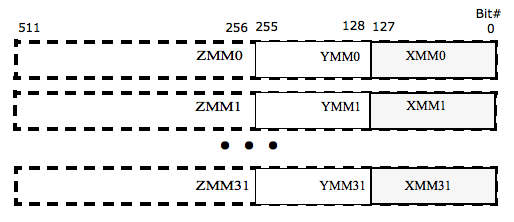
\includegraphics[width=\linewidth]{avx_mms.png}
    \caption{AVX-512 Bits Wide Vectors and SIMD Register Set}
    \label{fig:avx_mms}
\end{figure}

\arm also announced the new Armv8 architecture embraced \sve - a vector extension for AArch64
execution mode for the A64 instruction set of the
Armv8 architecture~\cite{arm-v8-ref, ARMv8-Architecture}.
%arm-v8-sve,
Unlike other SIMD architectures, \sve does not define the size of the vector
registers, instead it provides a range of values which permit vector code to
adapt the vector length at runtime with the feature of \emph{Vector Length
Agnostic} (VLA) programming~\cite{Advanced-SIMD,vla-stencil}. Vector length
constrains are in the range from a minimum of 128 bits up to a maximum of 2048
bits in increments of 128 bits. The first processor to support these
capabilities was released by Fujitsu and was named A64FX~\cite{fujitsugit}. It
has 48 calculation cores and two or four assistant cores. In addition, it can
perform single-precision and half-precision floating-point calculations, as well
as 8-bit and 16-bit calculations with 512-bit wide SIMD.

The Message Passing Interface (\mpi)~\cite{mpi-forum} has been a popular
parallel programming model for distributed memory systems, widely used in
scientific applications for the last couple of decades. In addition to its many
communication focused capabilities, MPI transcend the use of contiguous buffer
and allows the programmer to describe the memory patterns involved in
communications.
%
Many scientific applications operate on and communicate with rich and
non-contiguous memory layout patterns, which poses challenges to MPI
implementors dealing with complex data movements expected to achieves a high
percentage of the peak bandwidth.
% However, \mpi has been very successful in implementing regular, iterative
% parallel algorithms with well-defined communication behaviors. Data-driven
% applications often pose challenges associated with dealing with contiguous and
% non-contiguous data. These issues are harder to address with a traditional
% message-passing programming paradigm.
\mpi offers a mechanism, the derived datatype, to specify arbitrary,
regular and irregular memory layouts for sending and receiving messages for all
types of communications, one-sided (Remote Memory Access) or two-sided
(point-to-point and collective) communications. This powerful mechanism allows
integrating communication into the parallel algorithm and data layout and is
has become an essential part of application development and optimization.
%
Datatypes provides an abstract and versatile interface to specify arbitrary data
layouts and a portable, high-performance abstraction for data. We cover more in
details the different memory patterns support provided by \mpi in
\ref{ssec:datatypes}.

% As we mentioned, new architectures and processors provide more opportunities
% for \mpi libraries, which enables \mpi implementations to take advantage of
% those new features to be carefully designed to deliver the best possible
% performance for different communication primitives to the end application.

Communication-oriented point-to-point and collective operations dealing with
non-contiguous require intensive memory resources, as only part of the memory
fetched and prefetched by the hardware will be used during the communication. As
a result  the memory bandwidth become a bottleneck and limit the communication's
performance.
%
However, the presence of advanced architecture technologies introduced with wide
vector extension and specialized arithmetic operations, provides new
opportunities to minimize the impact of the irregular memory accesses but calls
for \mpi libraries to provide state-of-the-art design for advanced vector
extension (\sve and AVX-512).

This paper tackles the challenges of providing efficient support for irregular
memory accesses in the context of MPI datatypes and performs an extensive study
of the novel gather and scatter feature from AVX-512 and its applicability for
\mpi datatype communication.
%
More precisely, our design optimizes the pack and unpack operations for structured
data after datatype engine preprocessed the recursive or nested datatypes. We
have implemented and evaluated our strategy in the \ompi \mpi implementation.
% to provide our optimized \mpi datatype pack and unpack operation to speed
% up the communication that deals with non-contiguous small blocks datatype.
To summarize, this paper makes the following contributions:
%\begin{compactenum}
\begin{enumerate}
%
  \item evaluate the AVX-512 gather load and scatter store instructions as a mean
  to optimize the packing and unpacking operation for non-contiguous datatype
  using related intrinsic;
%
  \item demonstrate the efficiency of gather and scatter instructions in our
  implementation by performing extensive benchmarking experiments and analysis
  using this work in \ompi on a local cluster with Intel Xeon processor that
  supports AVX-512;
%
  \item demonstrate the efficiency of the approach with two popular applications
  in scientific computing: Stencil and 2D-FFT, strengthening the performance
  benefit from of design and implementation. This provides valuable insight and
  guideline on how long vectors can be used in high-performance platforms and
  software.
\end{enumerate}
%\end{compactenum}

The rest of this paper is organized as follows.
%
Section~\ref{sec:related} presents related efforts taking advantage of long
vector extension from Intel and Arm for different applications and libraries,
together with a survey of existing work about \mpi optimizations taking
advantage of novel hardware capabilities.
%
Section~\ref{sec:design} describes in details the design and implementation of
our optimized packing and unpacking methods in the scope of \ompi using AVX-512
intrinsic and instructions.
%
Section~\ref{sec:experiments} describes the performance difference between
default \ompi and \ourwork and provides a distinct insight into how the new
vector instructions can benefit \mpi.
%
Finally, Section~\ref{sec:application} illustrates the performance benefit we
get from \ourwork with two applications that demonstrate that our design and
implementation can speed up scientific applications, followed by the conclusion.

\begin{figure*}[ht]
  \centering
  % trim={<left> <lower> <right> <upper>}
  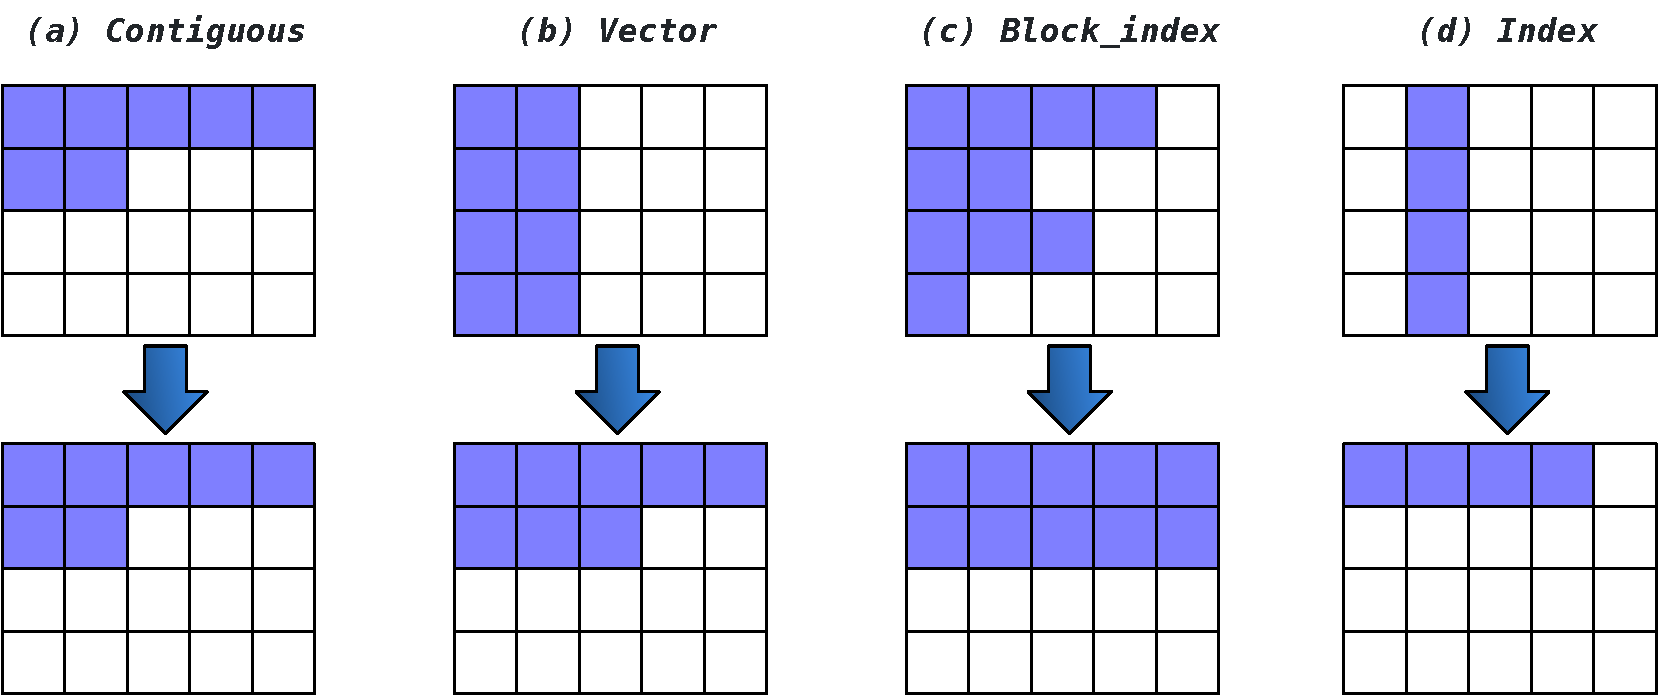
\includegraphics[width=0.8\linewidth]{ddt_ompi.pdf}
  \caption{Packing operation on different memory layout of datatype (contiguous and non-contiguous). The unpacking operation will do the exact opposite, scattering data from a packed, contiguous, buffer into the memory layout described in the \mpi datatype.}
  \label{fig:ddt_ompi}
\end{figure*}

\section{Related Work}\label{sec:related}

\todo{reorder to follow a logica path, from the upper layers to the lowest}
Taking advantage of processor's vector capabilities has a long track-record of
uses at all the level of software development.
%In this section, we survey related work on techniques taking advantages of
%advanced hardware or architectures.
%
Lim~\cite{Lim2018} explored matrix matrix multiplication based on blocked matrix multiplication
improves data reuse by data prefetching, loop unrolling, and the Intel AVX-512 to optimize
the blocked matrix multiplications.
%
Dosanjh et al.~\cite{tag-match} took advantage of using AVX vector operation for
\mpi message matching to accelerate matches demonstrating the efficiency
of long vectors.
%
This work~\cite{Berlin04} presented a new
zero-copy scheme to efficiently implement datatype communication over InfiniBand
scatter and gather work to optimize non-contiguous point-to-point communication.
%
Mellanox's InfiniBand~\cite{Gainaru2016} explored the use of hardware scatter
gather capabilities to eliminate CPU memory copies selectively and offload handling
data scatter and gather to the supported Host Channel Adapter. This capability is
used to optimize small data all-to-all collective.
%
In another work~\cite{sve-stencil}, they leveraged the characteristics of \sve to implement and optimize
stencil computations, ubiquitous in scientific computing, which shows
that \sve enables easy deployment of optimizations like loop unrolling,
loop fusion, load trading or data reuse.
%
This work~\cite{dongsve} explored the usage and performance of \sve vector instructions to optimize
memory access operation and reduction operation, simulation and benchmark results show that \sve
long instruction can speedup related operations. However, this work mainly used emulation tools to
study the performance benefits of such operation without further demonstration by experimenting
with applications.
%
Hashmi~\cite{ASHMI20201} proposed a Fast and low-overhead communication framework
for optimized zero-copy intra-node derived datatype communication on emerging CPU/GPU architectures.
%
%Hofmann~\cite{sparse-reduction} presented a pipeline algorithm for \mpi Reduce
%that used a Run Length Encoding scheme to improve the global reduction of sparse
%floating-point data.

Additionally, different techniques and
efforts have been studied to optimize \mpi communication operations.
%
Wu~\cite{wu2016} proposed GPU datatype engine that offloads the pack and unpack
work to GPU to take advantage of GPU's parallel capability to provide
high efficiency in-GPU pack and unpack.
%
Luo~\cite{luo-han} presented a new hierarchical autotuned collective communication
framework in \ompi, which selects suitable homogeneous collective communication
modules as sub-modules for each hardware level, and uses collective operations from
the sub-modules as tasks, and organizes these tasks to perform efficient hierarchical collective operations.
%
Zhong~\cite{avxop} explored the usage of long vector extension for reduction operation in \mpi, which
speedups the local computation in \mpi that directly benefits the overall performance of
collective reductions for applications.
%
Bayatpour~\cite{Bayatpour} proposed a hardware tag matching aware \mpi library and discusses various aspects and challenges of leveraging this feature in \mpi library. Moreover, it characterizes
hardware Tag Matching using different benchmarks and provides guidelines for the
application developers to develop Hardware Tag Matching-aware applications to maximize their usage of this feature.
%
Hjelm~\cite{Hjelm} described a new RMA implementation for \ompi. The implementation targets scalability
and multi-threaded performance. It describes the design and implementation of RMA improvements
and offers an evaluation that demonstrates scaling to 524,288 cores.

In this work we study the integration of vector gather/scatter capabilities
into the \mpi datatype engine, and provide a detailed analysis about the
potential efficiency gains.
%
Our approach takes advantage of Intel AVX512 instruction set, but the proposed
optimization is portable across all processors providing support for
gather/scatter instructions.

% general at the processor instruction level, which is more straightforward, and
% uses CPU resources only without external or extra hardware.

\section{Design and implementation in \ompi}\label{sec:design}

\begin{figure*}[ht]
  \centering
  % trim={<left> <lower> <right> <upper>}
  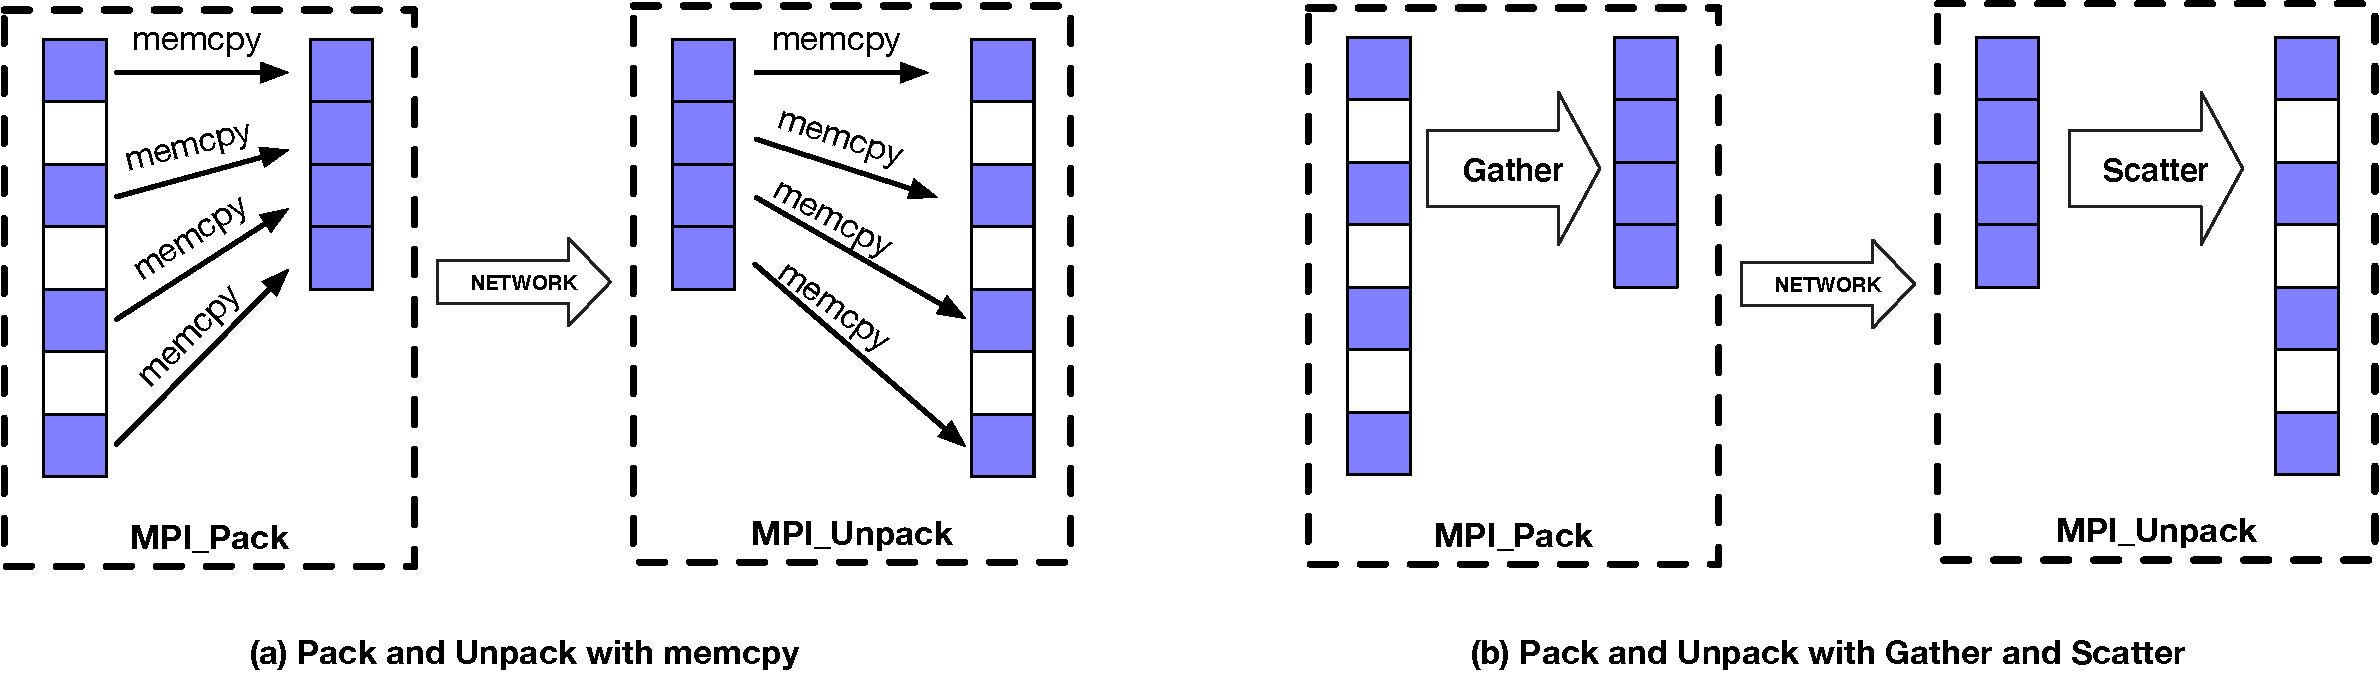
\includegraphics[width=0.9\linewidth]{send_recv_gs1.pdf}
  \caption{Comparison between general memory copy and AVX gather/scatter implementation for packing and unpacking}
  \label{fig:send_recv_gs1}
\end{figure*}

\subsection{Intel Advanced Vector Extension}

Intel Advanced Vector Extension (AVX) was a significant improvement to prior
Intel ISA, building upon the nascent set of vector instructions provided by the
MMX and SSE instructions set. Successive versions of the AVX instruction set
(AVX, AVX2, AVX-512) further increase the capabilities of the instruction set,
by adding support for additional operations (logical and bitwise), adding masked
operations, increasing the length of the vectors the operations apply onto, and
improve the memory accesses by providing larger and mnore complex load and store
to and from the vector registers.
% significant supports with longer vectors compared to 128-bits single
% instruction multiple data instructions. It supports the vast majority of
% previous generations' instructions to operate on 256- and 512-bits registers
% to support more powerful and efficient instruction.

AVX enhances broadcast, reduction and mask instructions to accelerate numerical
computations. Starting with The Haswell Intel micro-architecture support for the
256-bit AVX2 instructions implementing 256-bit data path with higher throughput.
Knights Landing processor extends this feature to more advanced 512-bit wide
registers.
%
AVX-512 provides enhanced functionalities for broadcast and add support for
permutation operations, vector reduction instructions, and instructions to
load/store contiguous and non-contiguous data elements from/to memory. It also
has more powerful packing capabilities with longer vectors, which can
encapsulate eight double-precision or sixteen single-precision floating-point
numbers, or eight 64-bit integers, or sixteen 32-bit integers within a vector.
Furthermore, it increases the performance for the most demanding computational
tasks by adding more vectors registers (32 vector registers, each 512 bits wide,
and eight dedicated mask registers), enhanced high-speed math instructions, and
introduces support for compact representation of large displacement value.

In this work we will take advantage of a small subset of the AVX-512
capabilities,
% AVX-512 supports more features that we intend to explore and use in this work,
such as operations on packed floating-point data or packed integer data, new
operations, additional gather/scatter support for non-contiguous memory access,
and the ability to have optional capabilities beyond the basic data type and
instruction sets.

\subsection{Memory access pattern}\label{ssec:datatypes}

Memory accesses are a critical component during communication, including
point-to-point and collectives as it defined the speed at which the data can be
made available for the network device.
%
Data need to be packed at the sender side before sending and be unpacked at the
receiver side. The datatype constructs provided by the \mpi standard provide
support for contiguous and non-contiguous memory layouts, allowing developers to
reason at a higher level of abstraction, thinking about data instead of focusing
on the memory layout of the data (for the pack/unpack operations). \mpi defines
data layouts of varying complexity that can be classified either as regular
(contiguous and regularly distributed such as a vector pattern defined by a
repetition count and a stride) or as irregular (with multiple constructors with
an increased level of irregularity, such as index and struct).

{\bf Contiguous} type is the simplest derived type: a number of repetitions of
the same datatype without gaps in-between, as shown in
Figure~\ref{fig:ddt_ompi}(a). C standard library provides function as memory
copy to manipulate the contiguous type. With the help of modern compilers, the
manipulation of such types can be converted directly into highly efficient
assembly code which is represented as a loop of load and store instructions
using vector registers.

For {\bf non-contiguous} datatype layouts, as shown in Figure~\ref{fig:ddt_ompi},
vector type Figure~\ref{fig:ddt_ompi}(b) is the most regular and certainly the
most widely used \mpi datatype constructor. Vector allows replication of a
datatype into locations that consists of equally spaced blocks, describing the
data layout using block-length, stride and count -- \emph{Block-length} refers
to the number of primitive datatypes that a block contains, \emph{stride} refers
to the number of primitive datatypes between blocks, and \emph{count} defines the
number of blocks that needs to be processed.
%
A distinctive flavor of vector datatype, frequently used in computational sciences
and machine learning, access a single column of matrix as presented in
Figure~\ref{fig:ddt_ompi}(d) and can be represented by a specialized vector type
with block-length equal one.

%
Other memory patterns continue to increase the irregularity of the vector
pattern by allowing the different components, \emph{block-length}, \emph{stride}
or \emph{displacement} and \emph{predefined type} to be represented as arrays of
values.
%
% Datatypes other than vector exposes even less regularity, and neither the
% size of each block nor the displacements between successive blocks are constant.
In order of growing complexity, \mpi supports INDEXED\_BLOCK (constant
block-length different displacements), INDEXED (different block-lengths and
different displacements), and finally STRUCT (different block-lengths, different
displacements, and different composing datatypes). Such datatypes
Figure~\ref{fig:ddt_ompi}(c) cannot be described in a concise format using only
block-length and stride.

\subsection{Pack and unpack with gather and scatter}

High-performance parallel algorithms and scientific applications often need to
communicate non-contiguous data. Without support for datatypes, applications
using non-contiguous memory layouts would need to pack the non-contiguous data
into a temporary contiguous buffer and send it to peer process. The receiver
would then perform the symmetric operation, the unpack, to distribute the data
from the contiguous receive buffer to the non-contiguous data buffer/memory.
However, this approach (known as ``Manual Packing/Unpacking”) limits the
communication performance because it requires several copies of the data,
increasing the memory footprint of the application but also the number of memory
copies in the communication critical path.
% Also, application developer needs to manage those temporary buffers manually,
% leading to poor productivity.
This packing/unpacking process requires considerable time. A previous
study~\cite{mpi-ddt-benchmark} has shown that packing and unpacking data could
take 90\% of the total communication overhead for non-contiguous sends and
receives. It is essential for \mpi community to provide efficient \mpi datatype
communication, reducing or removing the packing/unpacking overhead for
non-contiguous data. To solve this problem, \mpi derived datatype provides the
convenience of hiding the complexity of sending non-contiguous data from
application developers, and moves the burden of efficient pack/unpack operations
from the application developers onto the \mpi library implementors.

Figure~\ref{fig:send_recv_gs1} give an overview of \ourwork transferring non-contiguous data
by using the gather and scatter feature from long vector extension in packing and unpacking, respectively.
For the default memory copy based packing/unpacking scheme, each segment of the data is copied into a pack
buffer and transferred to the receiver, the receiver then copies the data segment by segment into a distributed memory.
The gather and scatter scheme, on the other hand, on the sender side it replaces multiple small memory
copies by single gather instruction to fetch/load data from different memory addresses.
On the receiver side, it uses single scatter instruction to replaces multiple small memory
copies to distribute/store data into different memory addresses.

The detailed gather load and scatter store instruction for non-contiguous
small block data is revealed in Algorithm~\ref{fig:gs_algorithm}.
In this optimized algorithm, we can see for the ``gather\_pack" procedure, we use
intrinsic \emph{\textit{\_mm512\_type\_gather\_type (Src, ..., offsets, ...)}} to load data from
different memory addresses based on offsets to a single long vector, and then store it into our destination.
To be noted, for each vector type we only need to generate the offsets once, and repeatedly use this for all gather instructions.
For the ``scatter\_unpack" procedure, we first load the packed contiguous data to a long vector and then use the intrinsic
\emph{\textit{\_mm512\_type\_scatter\_type (Dst, ..., offsets, ...)}} to store the data to non-contiguous addresses.
For the remaining blocks with total size smaller than vector length, we explicitly use mask load and store operation to partially load/store the data from/to memory to maintain the integrity and correctness of our data.
This highly expands the limited performance of memory operations for small non-contiguous memory blocks. To be noted,
this strategy primarily benefits datatypes with small block size, which requires at least two or more blocks can be encapsulated
within a single long vector.

\todo[inline]{the interest of the algorithm in \ref{fig:gs_algorithm} is more
than questionable. First it indicates that the only datatype supported with
gather/scatter operations would be a vector type, and this is, at least from the
paper perspective, more than restricted). Second, it doesn't even correctly
track the src and dst locations for the blocklen larger than the threshold. The
way the paper is written right now, the only contribution in it, except for the
benchmarking and testing, is this, the replacement of pack/unpack for short
vectors by gather/scatter operations. How would you evaluate the work involved
in all this ?}

\begin{algorithm}%[t]
\caption{Gather/Scatter based pack and unpack algorithm}\label{fig:gs_algorithm}

\textbf{\textit{vector\_bytes}} \Comment{Vector length in bytes}\\
\textbf{\textit{blocklen}} \Comment{Block length in bytes}\\
\textbf{\textit{threshold}} \Comment{Threshold to pick gather/scatter or memcpy based algorithm, calculated by block length and vector length}\\
\textbf{\textit{blocks\_in\_vl}} \Comment{Number of blocks can be packed in single vector}\\
\textbf{\textit{off\_sets}} \Comment{Offsets of elements to be packed in a single vector, calculated by address, block length and extend}\\
\textbf{\textit{load\_mask}} \Comment{Mask for partial load/store}\\ \vspace{0.5 cm}
\begin{algorithmic}[1]

\Procedure{Gather\_pack}{ $Count, Blocklen, Extend$ }
\If {( $blocklen$ $\geqslant$ threshold )}
    \For { $k \gets 0$ to $Count$ }
      \State {memcpy(blocklen,Src,Dst)}
    \EndFor
\Else
  \State $blocks\_in\_vl$ = vector\_bytes / $blocklen$
  \State Generate $offsets$
  \For { $k \gets 0$ to ($Count$ / $blocks\_in\_vl$) }
    \State \_mm512\_type\_gather\_type (Src, ..., offsets, ...)
    \State \_mm512\_store\_type(Dst, ...)
    \State update address
    \State update count
  \EndFor
  \State Generate $load\_mask$
  \State gather remaining blocks
\EndIf
\EndProcedure
\end{algorithmic}
\begin{algorithmic}[1]

\Procedure{Scatter\_unpack}{ $Count, Blocklen, Extend$ }
\If {( $blocklen$ $\geqslant$ threshold )}
    \For { $k \gets 0$ to $Count$ }
      \State {memcpy(blocklen,Src,Dst)}
    \EndFor
\Else
  \State $blocks\_in\_vl$ = vector\_bytes / $blocklen$
  \State Generate $offsets$
  \For { $k \gets 0$ to ($Count$ / $blocks\_in\_vl$) }
    \State \_mm512\_load\_type(..., Src)
    \State \_mm512\_type\_scatter\_type (Dst, ..., offsets, ...)
    \State update address
    \State update count
  \EndFor
  \State Generate $load\_mask$
  \State scatter remaining blocks
\EndIf
\EndProcedure
\end{algorithmic}
\end{algorithm}

We implemented our AVX-512 based pack and unpack operation work in the \ompi
datatype engine. \ompi is based on a Modular Component
Architecture~\cite{dong_prrte,gabriel04ompi} providing simple strategies for
extending or substituting the core subsystem with new features. As shown below,
we added our AVX-512 optimization work in the lowest level (OPAL) of \ompi
architecture that implements all datatype related operations with AVX-512 long
vector instructions as in Figure~\ref{fig:avx_mca}; also we integrate our new
code to automatically detect the hardware information to enable the AVX-512
feature or fallback to the default basic module if it is not supported by the
processor as show in Figure~\ref{fig:512flow}. To be noted, this component can
be extended out the scope of the generic pack and unpack operations.
%
\todo{the MCA Figure~\ref{fig:avx_mca} is unnecessary, as it does not provide
any added value to the paper}

\begin{figure}[h]
    \centering
    % trim={<left> <lower> <right> <upper>}
    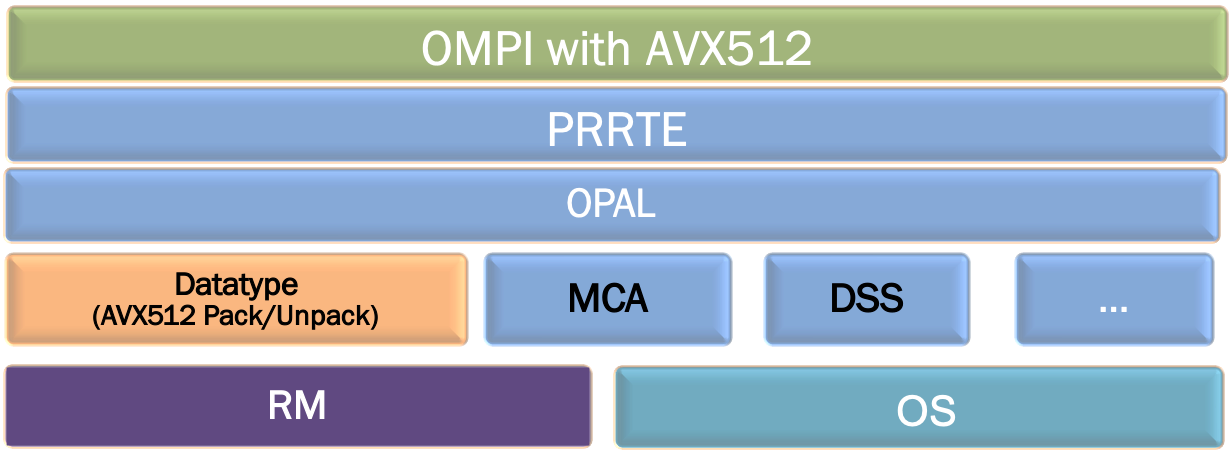
\includegraphics[width=\linewidth]{ompi-mca.png}
    \caption{\ompi architecture. The orange box represent Datatype component under OPAL. We added our AVX-512 gather pack and scatter unpack feature in this component.}
    \label{fig:avx_mca}
\end{figure}

\begin{figure}[h]
    \centering
    % trim={<left> <lower> <right> <upper>}
    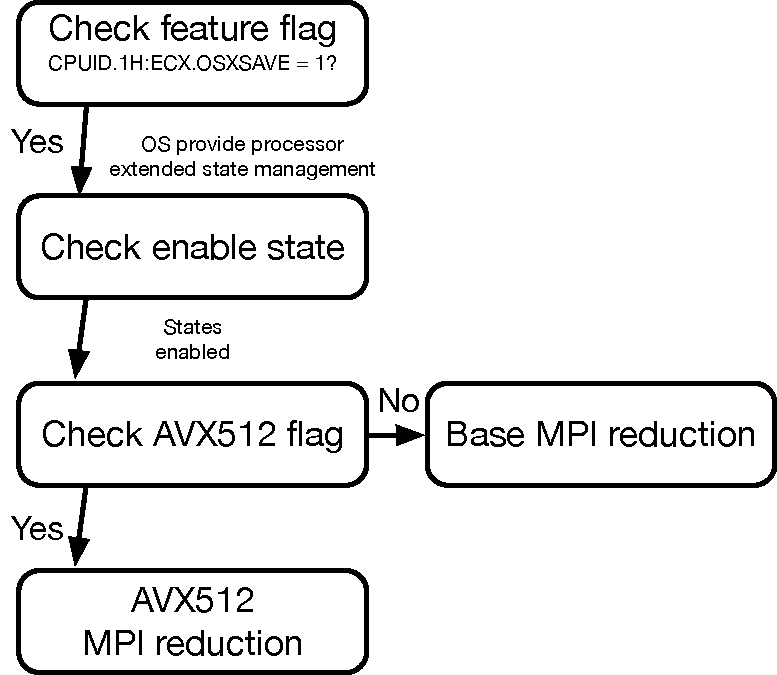
\includegraphics[scale=.45]{512-flow.pdf}
    \caption{Integrate and automatically activate the AVX-512 pack and unpack into the \ompi build system}
    \label{fig:512flow}
\end{figure}

\section{Benchmark evaluation}\label{sec:experiments}
Experiments are conducted on a local cluster, an Intel(R) Xeon(R) Gold 6254 based server running
at 3.10 GHz. The CPU consists of 18 physical cores, which support advanced features with cpu-flags  AVX-512 Foundation (avx512f) and AVX-512 Vector Length (avx512vl), new instruction set extensions, delivering wide (512-bit) vector operations capabilities,
with up to 2 FMAs (Fused Multiply Add instructions).

Our work is based upon \ompi master branch, git commit hash \#406bd3a~\cite{ompigit}. Each experiment
has been repeated at least 30 times, and we present the average. \todo{why not having also the standard deviation ?} We use a single node for all benchmark experiments.
This section compares the performance of \mpi pack and unpack operation with two implementations.
The \ompi default version uses general memory copy method during pack and unpack operation for non-contiguous datatypes.
It uses a for loop to copy all the blocks for a non-contiguous datatype.

\todo{why do you repeat this, it has been already described multiple times, and it is not like you are changing your work in the experimental section}
In the new implementation, we use the AVX-512 vector gather feature
for packing operation; on the receiver side, we use AVX-512 scatter feature for unpacking.
For the pack and unpack benchmark, we use the official test \textbf{to\_self} in \ompi repository
to perform packing and unpacking operation for a vector datatype with different message sizes.

\begin{figure}[h]
    \centering
    % trim={<left> <lower> <right> <upper>}
    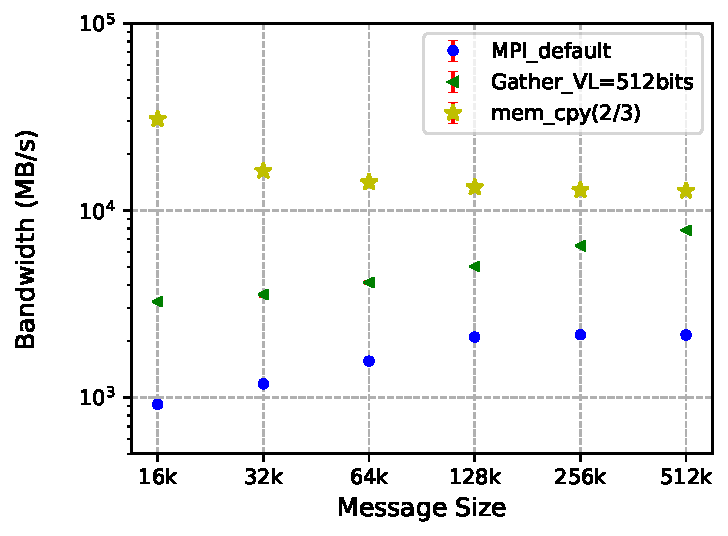
\includegraphics[width=\linewidth]{to_self_avx_gather_20tests_with_memcpy.pdf}
    \caption{Performance of MPI\_Pack for a vector datatype with the 2 implementations (classical memory copies and AVX-512)}
    \label{fig:gather20}
\end{figure}

\begin{figure}[h]
    \centering
    % trim={<left> <lower> <right> <upper>}
    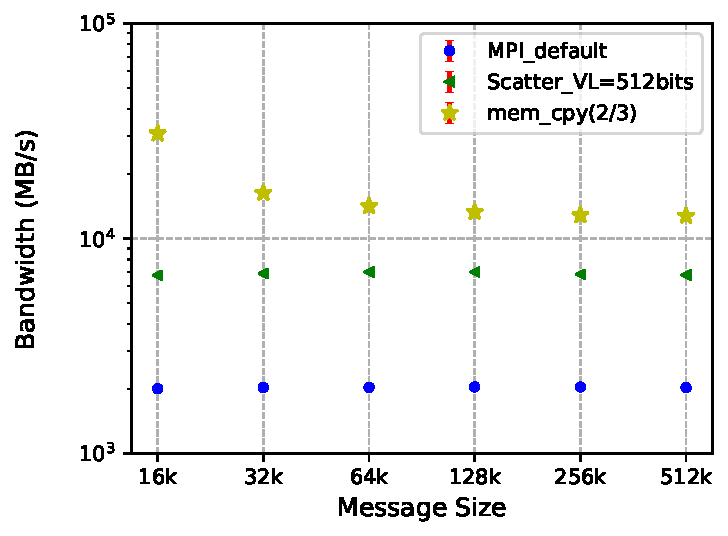
\includegraphics[width=\linewidth]{to_self_avx_scatter_20tests_with_memcpy.pdf}
    \caption{Performance of MPI\_Unpack for a vector datatype with the 2 implementations (classical memory copies and AVX-512)}
    \label{fig:scatter20}
\end{figure}

\begin{figure*}[h]
\centering
\begin{minipage}{.45\textwidth}
  \centering
  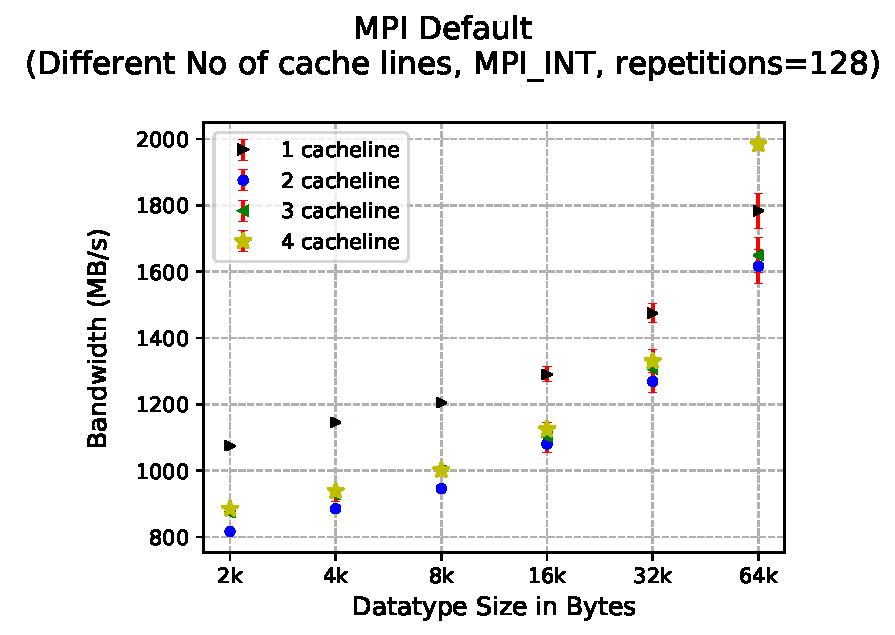
\includegraphics[trim={0 0.7cm 0 1.5cm},clip,width=\linewidth]{to_self_avx_gather_20tests__default_cachelines.pdf}
  {(a) Default MPI\_Pack}
\end{minipage}\vspace{0.5cm}
\begin{minipage}{.45\textwidth}
  \centering
  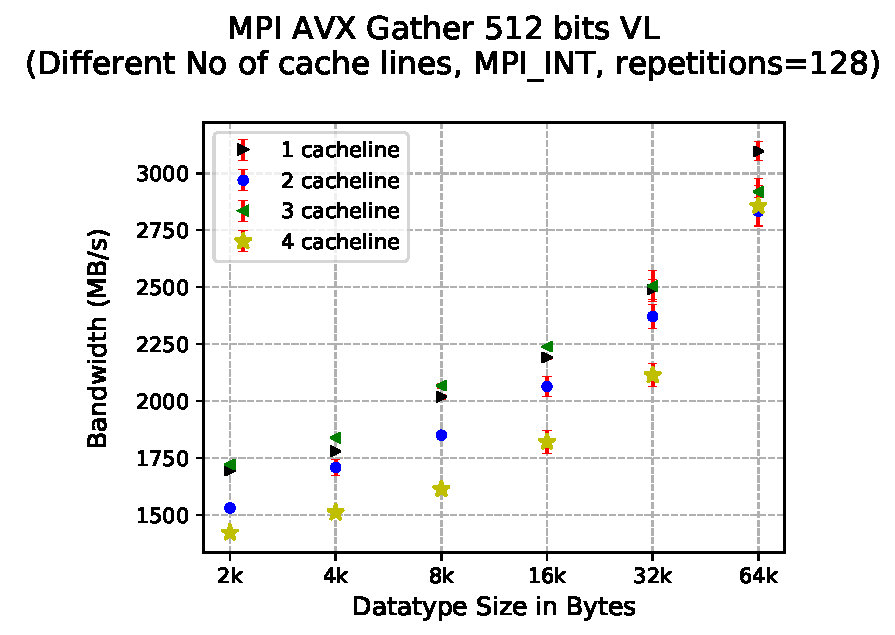
\includegraphics[trim={0 0.7cm 0 1.5cm},clip,width=\linewidth]{to_self_avx_gather_20tests_cachelines.pdf}
  {(b) Gather MPI\_Pack}
  %\vspace*{-0.7cm}\hspace*{0cm}\textcolor{black}{}
\end{minipage}
\centering
\begin{minipage}{.45\textwidth}
  \centering
  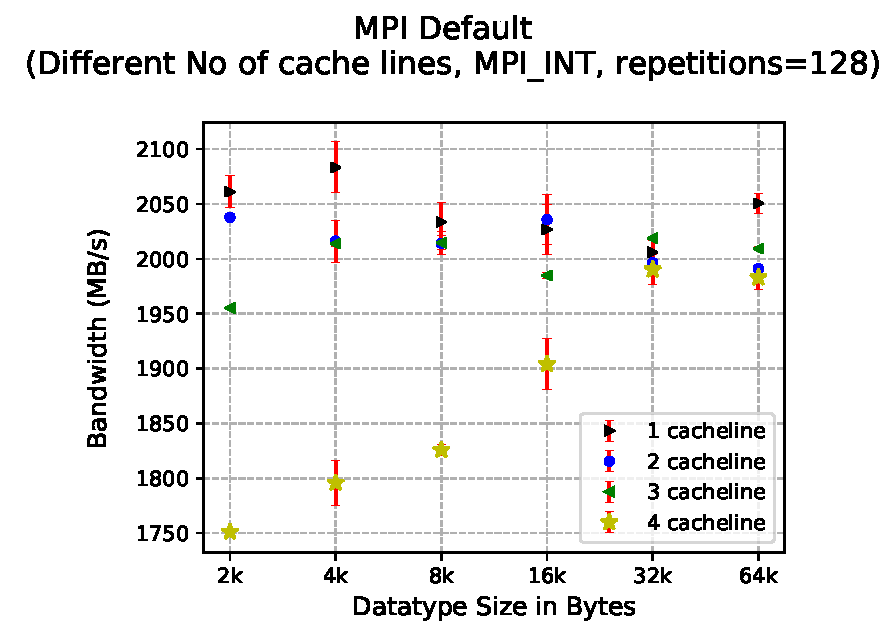
\includegraphics[trim={0 0.7cm 0 1.5cm},clip,width=\linewidth]{to_self_avx_scatter_20tests__default_cachelines.pdf}
  {(c) Default MPI\_Unpack}
\end{minipage}%
\begin{minipage}{.45\textwidth}
  \centering
  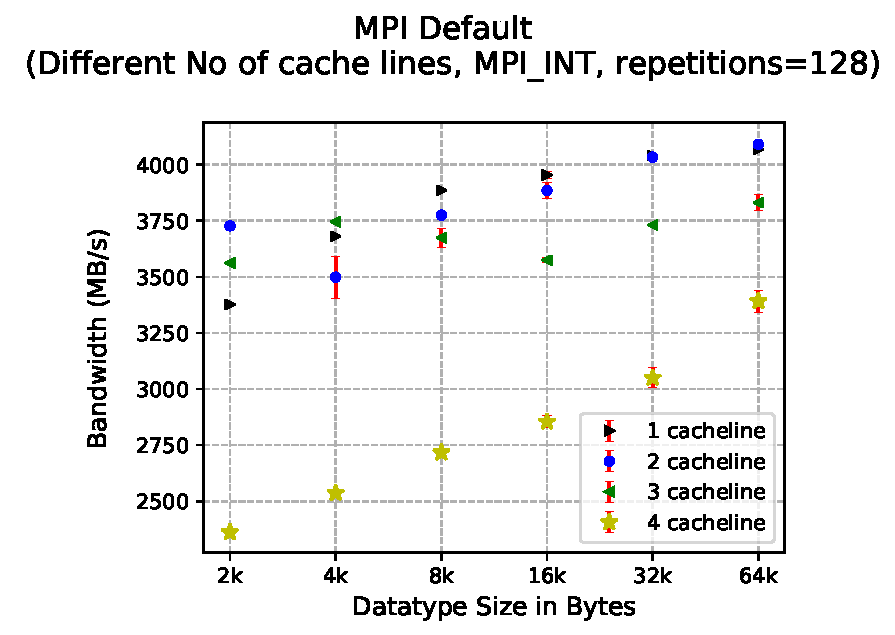
\includegraphics[trim={0 0.7cm 0 1.5cm},clip,width=\linewidth]{to_self_avx_scatter_20tests_cachelines.pdf}
  {(d) Scatter MPI\_Unpack}
  %\vspace*{-0.7cm}\hspace*{0cm}\textcolor{black}{}
\end{minipage}
\captionof{figure}{Pack and unpack across different number of cache-lines}
\label{fig:cachelines}
\end{figure*}

We compare the packing and unpacking performance separately to highlight the
benefit we get from gather load and scatter store. For the experiments, we use a
vector datatype with primitive datatype MPI\_INT constructed with $block length
= 2, gap = 1, count = 1024$, which means we pack two out of three integers for each
repetition. Figure~\ref{fig:gather20} displays the performance comparison
between \ompi default packing algorithm and AVX-512 gather packing algorithm.
The X-axis shows the size of the packed buffer; Y-axis shows the actual
bandwidth we get, which means the higher the better. We can see that by using
gather feature our optimized packing strategy achieves $2.3 \sim 3.5$ times
speedup. We also compare together with memory copy for contiguous data, which
indicates the peak memory bandwidth. We can see that even for non-contiguous
data, when the message size increased to 512KB, we achieve 41\% of the peak
bandwidth. Figure~\ref{fig:scatter20} presents the performance comparison
between \ompi default unpacking algorithm and AVX-512 scatter unpacking
algorithm. We can see that by using scatter feature our optimized unpacking
strategy achieves 3.4 times speedup. Comparing to memory copy bandwidth, our
scatter method achieve 35\% the performance of peak bandwidth. We can see that
unpacking acquires less efficiency than packing when compare to peak bandwidth
from memory copy, which is because reading from non-contiguous addresses is more
efficient than writing to non-contiguous addresses. Also, compared to contiguous
memory copy, gathers and scatters require the hardware to do more work than
contiguous SIMD loads and stores, and are likely to access more cache
lines/pages (depending on the specific access pattern). This will cause higher
instruction overheads. To be noted, for the memory copy operation we only copy
two-thirds the data size of the total unpacked buffer.

To further explore and understand the behavior of non-contiguous data movement during pack and unpack operation,
we conducted experiments with different gap length between blocks. This is because with different memory layouts and patterns, vectorization efficiency is not always as expected. Also, we want to investigate gather and scatter capability across cache lines. Generally speaking, gathering and scattering data cross cache lines reduces the effective memory bandwidth.
We want to study if our gather and scatter optimization maintains good efficiency with a more complex memory layout.
For our test platform, the cache line size is 64-bytes. We tested with vector datatype with block length fixed to one for MPI\_INT, and then we vary the stride to different cache line sizes ($1 \sim 4$) for both pack and unpack.

Figure~\ref{fig:cachelines} shows the result for the \mpifunc{Pack} and \mpifunc{Unpack} with MPI default and \ourwork.
Our optimization using intrinsic, which gives us complete control of the low-level details at the expense of productivity and portability.
Overall, for both gather and scatter results demonstrate that with AVX-512 enabled operation it is faster than memory copy operation with different stride size cross cache lines.

To be more specific, comparing MPI default Figure~\ref{fig:cachelines}(a) with gather pack Figure~\ref{fig:cachelines}(b) we noticed two aspects, (1) the performance for both implementation decreases as stride increases. One possible reason could be that data being gathered spread across multiple cache lines; software typically tests the completion mask to see if all elements have been read, and if not, loops back and re-executes the instruction. Consequently, the performance of a gather operation decreases as the distance (in memory) between data being gathered increases.
(2) Both implementations show performance slowdown but with different trends.
We can see that memory copy has a significant performance reduction when the stride increased to across two cache lines. However, for the gather results the decrease is trivial.
Also, the trend for memory copy performance decreases immediately after increased the stride longer than a single cache line.
Moreover, for the gather pack case, the reduction is gradual.
For the unpacking operation, overall, it shows the same trend as packing, which shows performance decrease as stride increases. Furthermore, the speedup gain from scatter seems more evident than gather.

\section{Application Evaluation}\label{sec:application}

\begin{figure*}[h]
    \centering
    % trim={<left> <lower> <right> <upper>}
    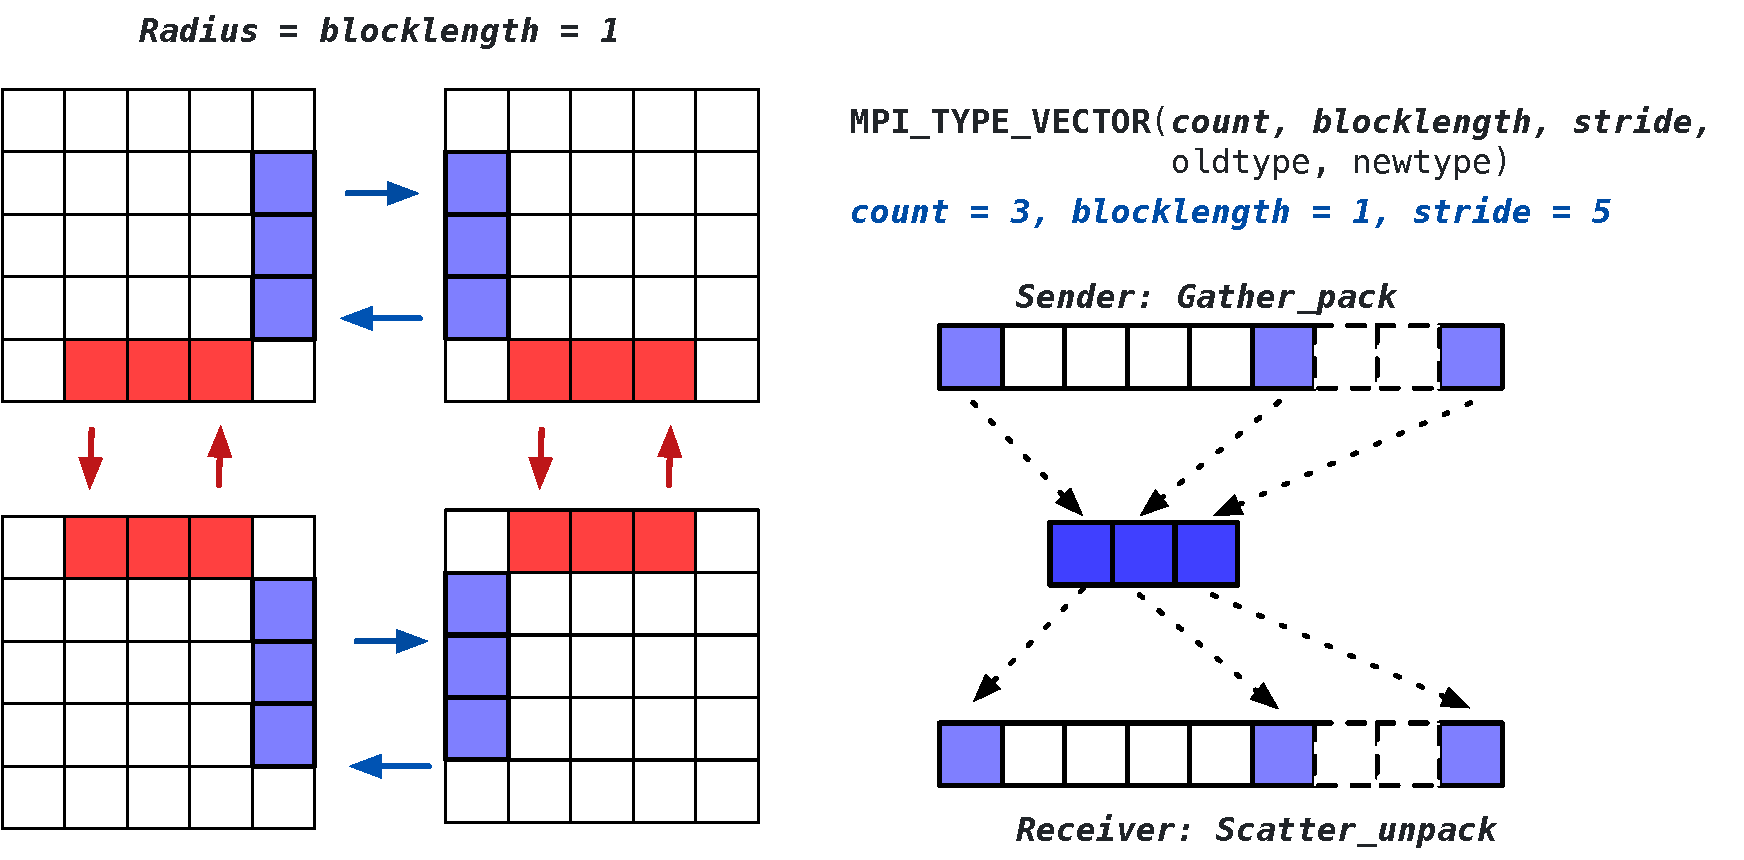
\includegraphics[trim={0 0 0 1.5cm},clip, width=0.9\linewidth]{stencil3.pdf}
    \caption{Domain-decomposed 2D stencil. Data exchanged in east-west direction must be packed and unpacked in communication}
    \label{fig:stencil3}
\end{figure*}

\subsection{Domain-decomposed 2D stencil}\label{sec:stencil}
Stencil computation is an important and fundamental algorithm
used in a large variety of scientific simulation applications.
Stencil codes are most commonly found in the codes of computer
simulation in the context of scientific and engineering HPC applications.
It involves a large number of iterations,
in each of which the value of every element in a matrix is
updated using values of its neighbors.

A 2D five-point stencil is a stencil made up of the point itself
together with its four ``neighbors", each point has four neighbors: up, down,
left and right, as shown in Figure~\ref{fig:stencil3}, we can see that the global
domain is represented by an N*N two-dimension matrix,
which gets partitioned into multiple blocks (one per process) of roughly equal size.
After each computation step, the boundary regions of
these partitions have to be exchanged with its four neighboring processes
before the next time-step can be started.
For easy explanation, we assume matrices are stored in ``Row Major" order,
data exchanged in the north-south direction is a contiguous pattern.
In contrast, the data exchange in the east-west direction is a non-contiguous pattern.
There are two ways to handle the communication: the first one is to send and receive the
data in multiple small chunks, which can be inefficient due to the constant overhead associated
with each send operation; The second method is that the data has to be
packed into a consecutive buffer and sent in one piece. On the receiver side,
this process has to be reversed (the data has to be
unpacked) after such data is received.

We can see that \ourwork can speed up the packing and unpacking procedure for this east-west
direction communication. We use gather and scatter to pack and unpack the boundary regions.
For the east-west boundary it can be represented with a vector datatype, as shown in Figure~\ref{fig:stencil3}.
For this particular vector type it is constructed as show in table~\ref{tab:ewvector} below.
\begin{table}
  \centering
  \caption{East-west vector data represent}\label{tab:ewvector}
  \small
  \begin{tabular}{cclll}
    \toprule
    \midrule
      \texttt{\bf Blocklen} & Radius \\
      \texttt{\bf Stride} & Number of Columns for each partitioned data set \\
      \texttt{\bf Count} & Number of Rows for each partitioned data set - 2 \\
      \bottomrule
  \end{tabular}
\end{table}

\begin{table}[h]
  \centering
  \caption{\mpi stencil configuration and execution on 2D grid}\label{tab:ewconfig}
  \small
  \begin{tabular}{cclll}
    \toprule
    \midrule
      \texttt{\bf Number of ranks} & 16 \\
      \texttt{\bf Grid size} & 1000 \\
      \texttt{\bf Radius of stencil} & 1, 2, 3 \\
      \texttt{\bf Tiles in x/y-direction} & 2/8 \\
      \texttt{\bf Type of stencil} & Star \\
      \texttt{\bf Data type} & Single precision \\
      \texttt{\bf Number of iterations} & 100 \\
      \bottomrule
  \end{tabular}
\end{table}

\begin{figure}[h]
    \centering
    % trim={<left> <lower> <right> <upper>}
    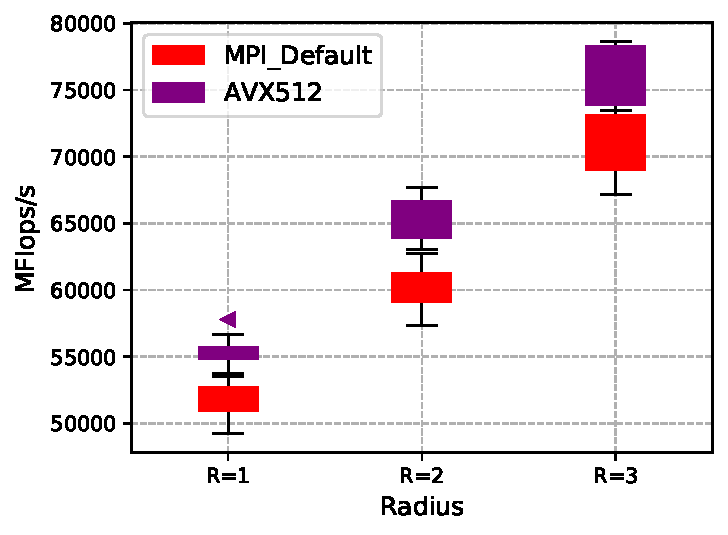
\includegraphics[width=\linewidth]{stencil_diff_radius.pdf}
    \caption{2-d Stencil results with and without AVX-512 gather pack and scatter unpack for different radius}
    \label{fig:stencil_diff_radius}
\end{figure}

In this section we investigate the performance benefit of \ourwork against default \ompi.
The application benchmark is based on the Stencil \mpi implementation from Parallel
Research Kernels (PRK)~\cite{mpistencil,PRK2014} -- are a suite of simple kernels for the study of the efficiency
of distributed and parallel computer systems, including all software and hardware components that make up the system.
They cover a wide range of common parallel application patterns, especially from the area of HPC.
This stencil implementation uses a for loop with memory copy function to pack the chunks for the non-contiguous data from east-west boundary.
We optimized this packing implementation with the vector representation we described above.

We conducted our experiment on the same Intel Xeon Gold6254 based cluster. Table~\ref{tab:ewconfig} shows our experiment configuration for this stencil application.
We executed our experiments with 16 processes with different processes grid arrangements and achieved
similar results, here we present to show the result with process arrangement as 2*8 in x/y direction.
The stencil is a five points stencil using single precision executed for 100 iterations.
We demonstrate the effectiveness of \ourwork with three tests using different radius. As demonstrated in Figure~\ref{fig:stencil_diff_radius} we compared the performance of two implementations. We see that our gather and scatter
optimized implementation decreases the packing and unpacking cost for communication during each computation step.
Consequently, we improved collective operation that drives up the overall application performance by 10\% for all three cases.
We expect the performance benefit continues for 3D stencil applications and could be even more obvious. Because for 3D
stencil, each node needs to communicate with eights neighbors, and six of those communications use non-contiguous datatype.

%MPI stencil execution on 2D grid
%Number of ranks        = 16
%Grid size              = 1000
%Radius of stencil      = 3
%Tiles in x/y-direction = 2/8
%Type of stencil        = star
%Data type              = single precision
%Compact representation of stencil loop body
%Number of iterations   = 100


\begin{figure}[h]
    \centering
    % trim={<left> <lower> <right> <upper>}
    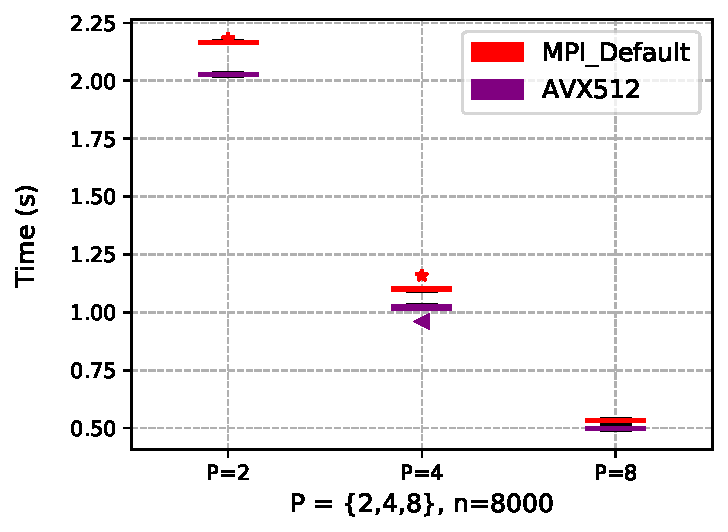
\includegraphics[width=\linewidth]{fft2_diff_p1.pdf}
    \caption{2-d FFT results with and without AVX-512 gather pack and scatter unpack for different number of processes}
    \label{fig:fft2_diff_p}
\end{figure}

\subsection{2D Fast Fourier Transform}\label{sec:FFTs}
The Fast Fourier Transform (FFT) is one of the most significant algorithms for exascale applications in science and engineering across various disciplines. Applications range from image analysis
and signal processing to the solution of partial differential equations through spectral methods.
Also, diverse parallel libraries exist that rely on efficient FFT computations, particularly in particle applications ranging from molecular dynamics computations to N-Body simulations. Thus, for all these applications, it is essential to have
access to a fast and scalable implementation of an FFT
algorithm, an implementation that can take advantage of efficient communication
library and component, and maximize these benefits for applications.
We aim to expand and demonstrate the performance advantages we integrated into \ompi that can benefit all-to-all
communication in FFT.

An FFT on multidimensional data can be performed as a sequence
of one-dimensional transforms along each dimension.
For example, a two-dimensional FFT can be computed by performing 1d-FFTs along both dimensions.
With multiple MPI processes, after each process computes the 1d-FFT, a matrix transpose needed to be performed
among MPI processes using MPI\_Alltoall operation. Also n-d FFTs can be computed
by performing 1-d FFTs in all n dimensions.
In this subsection, we examine the performance of our gather pack and scatter unpack approach,
we measured the performance (running time) of a micro-benchmark: 2D FFT Benchmark with code version~\cite{2dfft}.
More details about the implementation can be found in this paper~\cite{ddtHoefler}. To our interest of region, in this implementation it uses a vector type for the all to all communication.
We compare the performance of this all to all collective between \mpi default and our proposed optimized design.
% mentioned in this work~\cite{mpi-ddt-benchmark}

Figure~\ref{fig:fft2_diff_p} shows the performance comparison of the 2D FFT application completion time
between our AVX-512 enabled pack and unpack operation and the default operation in \ompi.
We tested with a different number of processes as show in X-axis. The number of elements in each dimension is 8000.
We can see that we achieve 8\% performance speedup under all three cases for the entire completion time.

\section{Conclusion}\label{sec:conclusion}
In this paper, we presented the benefits of using the new features from
Intel AVX-512 long vector extension. We evaluated the performance advantages
of the gather and scatter feature to load and store non-contiguous data layout.
Furthermore, based on our investigation and analysis, we designed and implemented
an optimistic \mpi optimization.
%

We introduced a new packing and unpacking strategy in the Datatype engine under OPAL
level in \ompi using AVX-512 intrinsic to speedup the communication for a non-contiguous datatype.
We demonstrated the efficiency of our new pack and unpack operation by a benchmark (\textbf{to\_self})
in \ompi repository. For a vector type ($blocklen = 2, gap =1$), we
achieve $2.3 \sim 3.5$ times speedup with gather pack and 3.5 times speedup with
scatter unpack. We also investigated gather and scatter across cache lines and achieved good performance.
To further validate the performance improvements, we conducted experiments with two applications: five-point Stencil and 2D-FFT. Our proposed designs outperforms default \ompi by 10\% and 8\%, respectively.

Our analysis and implementation of \ompi optimization provide useful insights and guidelines on how
novel long vector features could be used in high-performance computing platforms and
software to improve the efficiency of parallel libraries and applications.

%\section*{Acknowledgement}
\section{Acknowledgments}
%
This material is based upon work supported by the National Science Foundation under Grant No. (1725692); and the Exascale Computing Project (17-SC-20-SC), a collaborative effort of the
U.S. Department of Energy Office of Science and the National Nuclear Security Administration.

%\bibliographystyle{IEEEtran}
%\bibliography{./sample-base.bib}{}
\bibliographystyle{IEEEtran}
\bibliography{sample-base}

\end{document}

%%
%% End of file `sample-sigconf.tex'.
